\chapter{Type of Networks and Devices}

\section{Introduction}
In the modern digital world, computer networks form the backbone of communication, data exchange, and remote access. From accessing the internet on a mobile phone to sharing files within a college lab, networks are at the heart of nearly every interaction involving computers.

This chapter explores the various types of networks and the devices that enable them. By understanding how networks are classified—based on their size, architecture, and topology—we gain insight into their practical applications and limitations. We also look into the essential networking devices that help connect, control, and secure data flow across these networks.

\section{Type of Network (Based on Scale/Geography)}

\subsection{Personal Area Network (PAN)}
A Personal Area Network (PAN) is the smallest type of network, typically used for communication between devices in close proximity to an individual—usually within a range of 10 meters. It connects devices such as smartphones, tablets, laptops, headphones, or smartwatches using technologies like Bluetooth, USB, or infrared. PANs are commonly used for tasks like file sharing or peripheral connectivity (e.g., printing a document from a phone to a nearby printer).

\begin{figure}[H]
    \centering
    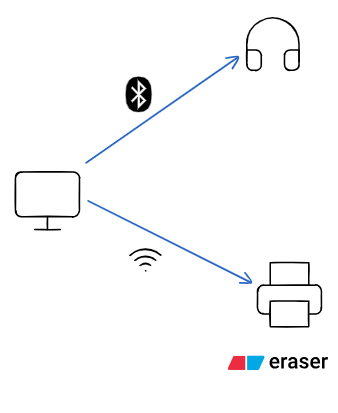
\includegraphics[width=0.3\textwidth]{images/chapter2/pan.png}
    \caption{Personal Area Network}
    \label{fig:pan}
\end{figure}


\subsection{Local Area Network (LAN)}
A Local Area Network (LAN) is used to connect computers and devices within a limited geographic area such as a home, office, or school. It enables resource sharing, such as printers, files, or internet connections, among connected devices. LANs offer high-speed data transfer and are usually managed using Ethernet cables or wireless technology. In academic institutions and small businesses, LANs are essential for internal communication and collaboration.

\begin{figure}[H]
    \centering
    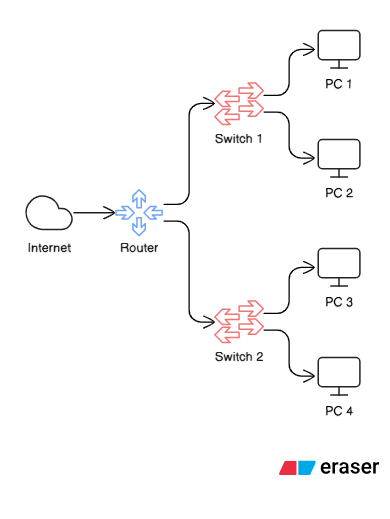
\includegraphics[width=0.3\textwidth]{images/chapter2/lan.png}
    \caption{Local Area Network - Within Same Building}
    \label{fig:lan}
\end{figure}


\begin{didyouknowbox}
Did you know that the first Ethernet LAN, invented by Robert Metcalfe in 1973, had a data rate of just 2.94 Mbps? Today, LANs easily reach 1 Gbps or more!
\end{didyouknowbox}


\subsection{Wireless LAN (WLAN)}
A Wireless Local Area Network (WLAN) functions similarly to a LAN, but uses wireless communication technologies like Wi-Fi instead of physical cables. WLANs provide the flexibility of mobility within the network coverage area, making them ideal for homes, coffee shops, and educational campuses. Devices connect through an access point, typically a wireless router, which manages data transmission within the network.

\begin{figure}[H]
    \centering
    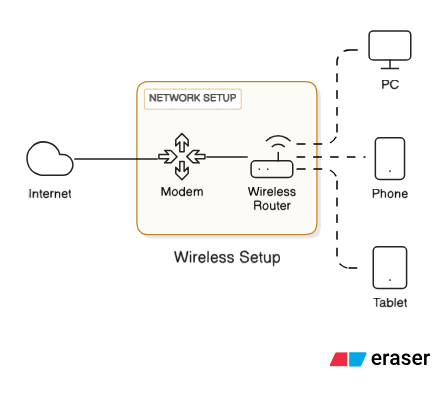
\includegraphics[width=0.5\textwidth]{images/chapter2/wlan.png}
    \caption{Wireless Local Area Network}
    \label{fig:wlan}
\end{figure}


\subsection{Metropolitan Area Network (MAN)}
A Metropolitan Area Network (MAN) spans a larger geographical area than a LAN, typically covering a city or a large campus. It connects multiple LANs together to form a network that can be managed centrally. MANs are often used by government agencies, educational institutions, and large companies to connect offices in different parts of a city. Fiber-optic cables or high-speed wireless technologies are commonly used for MANs.

\begin{figure}[H]
    \centering
    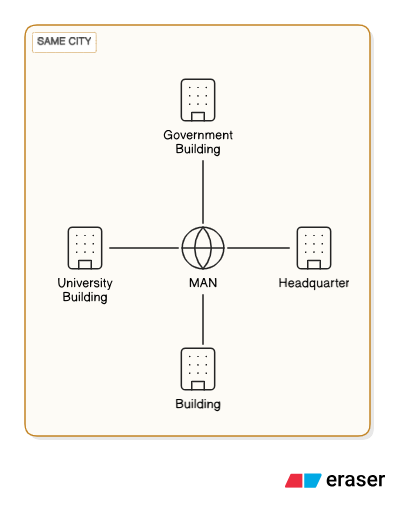
\includegraphics[width=0.3\textwidth]{images/chapter2/man.png}
    \caption{Metropolitan Area Network - Within Same City}
    \label{fig:man}
\end{figure}

\subsection{Wide Area Network (WAN)}
A Wide Area Network (WAN) connects computers and smaller networks over large geographical areas, such as cities, countries, or even continents. The most well-known example of a WAN is the Internet. WANs rely on telecommunications networks, satellite links, or undersea cables to transfer data across great distances. They are essential for multinational organizations, remote access to cloud services, and global communication.

\begin{figure}[H]
    \centering
    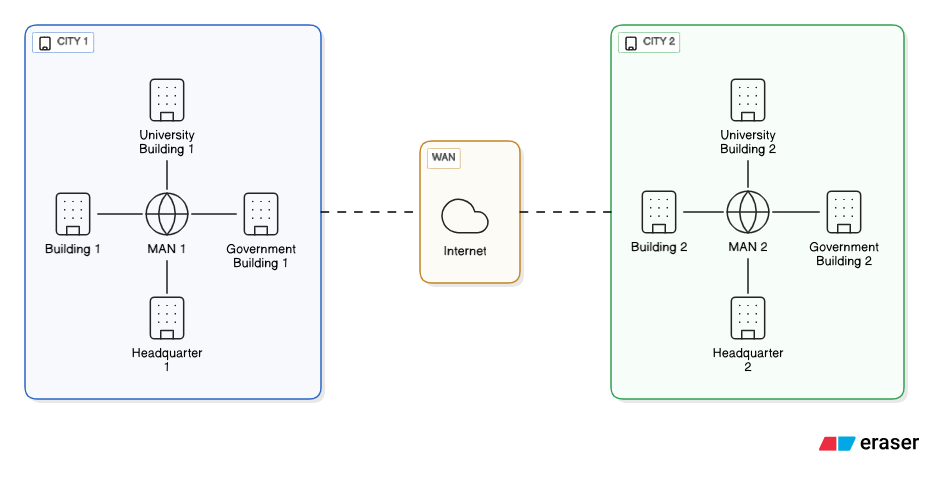
\includegraphics[width=0.8\textwidth]{images/chapter2/wan.png}
    \caption{Wide Area Network - Within Different Continents}
    \label{fig:wan}
\end{figure}

\subsection{Storage Area Network (SAN)}
A Storage Area Network (SAN) is a specialized high-speed network that provides access to consolidated, block-level data storage. It is commonly used in data centers and enterprise environments where large volumes of data need to be stored and accessed quickly and reliably. Unlike traditional networks, SANs are optimized for storage and provide faster performance and better data management.

\begin{figure}[H]
    \centering
    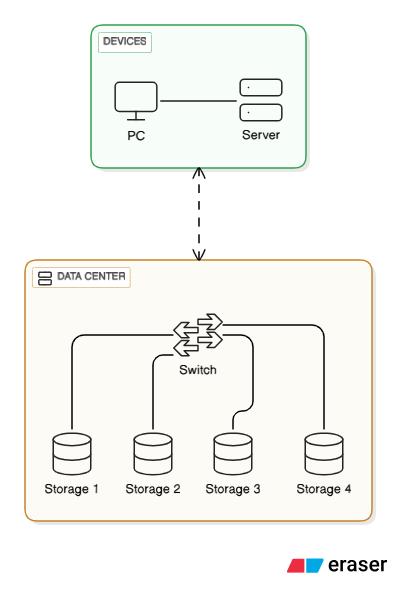
\includegraphics[width=0.5\textwidth]{images/chapter2/san.png}
    \caption{Storage Area Network - Within Data Center}
    \label{fig:san}
\end{figure}


\subsection{Virtual Private Network (VPN)}
A Virtual Private Network (VPN) creates a secure, encrypted connection over a public network—typically the Internet. It allows users to send and receive data as if their devices were directly connected to a private network. VPNs are widely used for remote work, secure browsing, and bypassing geo-restrictions. By masking IP addresses and encrypting data, VPNs provide privacy and protection from cyber threats, especially when using public Wi-Fi networks.


\section{Type of Network (Based on Architecture)}

\subsection{Client-Server Network}
A Client-Server Network is a centralized architecture where clients request services from a server. Common in businesses and institutions, it enables centralized control, resource sharing, and better security.

\begin{table}[H]
\centering
\caption{Client-Server Network: Advantages and Disadvantages}
\begin{tabularx}{\linewidth}{|X|X|}
\hline
\textbf{Advantages} & \textbf{Disadvantages} \\
\hline
Centralized control and management & Higher cost due to server hardware and maintenance \\
\hline
High security and backup capabilities & If the server fails, clients lose access to resources \\
\hline
Scalable and reliable performance & Requires specialized configuration and administration \\
\hline
\end{tabularx}
\end{table}

\subsection{Peer-to-Peer (P2P) Network}
In a Peer-to-Peer network, each computer acts as both a client and a server. It's suited for small-scale environments and direct resource sharing.

\begin{table}[H]
\centering
\caption{Peer-to-Peer Network: Advantages and Disadvantages}
\begin{tabularx}{\linewidth}{|X|X|}
\hline
\textbf{Advantages} & \textbf{Disadvantages} \\
\hline
Easy and inexpensive to set up & Difficult to manage as the number of devices increases \\
\hline
No need for a dedicated server & Less secure and reliable than client-server networks \\
\hline
Each device can share resources & Poor scalability under heavy load \\
\hline
\end{tabularx}
\end{table}

\subsection{Hybrid Network}
A Hybrid Network combines the features of both client-server and peer-to-peer models, offering flexibility and efficiency.

\begin{table}[H]
\centering
\caption{Hybrid Network: Advantages and Disadvantages}
\begin{tabularx}{\linewidth}{|X|X|}
\hline
\textbf{Advantages} & \textbf{Disadvantages} \\
\hline
Flexible and adaptable architecture & More complex to design and manage \\
\hline
Allows centralized control where needed & May require advanced configuration and planning \\
\hline
Efficient use of both local and centralized resources & Potential compatibility issues between models \\
\hline
\end{tabularx}
\end{table}



\section{Networking Devices}

Networking devices are essential components used to build and manage computer networks. Each device plays a specific role in data transmission, connectivity, and network security.

\subsection{Network Interface Card (NIC)}
\begin{itemize}[leftmargin=1.5cm]
  \item \textbf{Definition:} A hardware component that enables a device to connect to a network.
  \item \textbf{Purpose:} Acts as the interface between a computer and the network (wired or wireless).
  \item \textbf{Use Case:} Every desktop or laptop has a NIC to access LAN or Wi-Fi networks.
\end{itemize}

\subsection{Hub}
\begin{itemize}[leftmargin=1.5cm]
  \item \textbf{Definition:} A basic device that connects multiple devices in a LAN and broadcasts data to all of them.
  \item \textbf{Purpose:} Provides a central connection point in small networks.
  \item \textbf{Use Case:} Previously used in simple LAN setups, now largely replaced by switches.
\end{itemize}

\subsection{Switch}
\begin{itemize}[leftmargin=1.5cm]
  \item \textbf{Definition:} A device that connects multiple devices and forwards data to the intended recipient using MAC addresses.
  \item \textbf{Purpose:} Reduces unnecessary data transmission, improving network efficiency.
  \item \textbf{Use Case:} Commonly used in offices and labs to connect computers and printers.
\end{itemize}

\subsection{Router}
\begin{itemize}[leftmargin=1.5cm]
  \item \textbf{Definition:} A device that connects different networks and routes data using IP addresses.
  \item \textbf{Purpose:} Enables communication between a local network and external networks like the Internet.
  \item \textbf{Use Case:} Used in homes to connect devices to the internet.
\end{itemize}

\subsection{Modem}
\begin{itemize}[leftmargin=1.5cm]
  \item \textbf{Definition:} A device that converts digital data to analog signals and vice versa.
  \item \textbf{Purpose:} Allows digital devices to connect over analog telephone or cable lines.
  \item \textbf{Use Case:} ISPs provide modems to customers for internet access.
\end{itemize}

\subsection{Access Point (AP)}
\begin{itemize}[leftmargin=1.5cm]
  \item \textbf{Definition:} A device that provides wireless access to a wired network.
  \item \textbf{Purpose:} Extends wireless network coverage and enables device mobility.
  \item \textbf{Use Case:} Used in homes, offices, and schools to provide Wi-Fi.
\end{itemize}

\subsection{Repeater}
\begin{itemize}[leftmargin=1.5cm]
  \item \textbf{Definition:} A device that regenerates and amplifies signals over long distances.
  \item \textbf{Purpose:} Extends the range of a network signal without data loss.
  \item \textbf{Use Case:} Used in large buildings to improve Wi-Fi signal strength.
\end{itemize}

\subsection{Bridge}
\begin{itemize}[leftmargin=1.5cm]
  \item \textbf{Definition:} A device that connects and filters traffic between two network segments.
  \item \textbf{Purpose:} Divides a network into segments to reduce traffic and collisions.
  \item \textbf{Use Case:} Used in older Ethernet networks to connect different LANs.
\end{itemize}

\subsection{Gateway}
\begin{itemize}[leftmargin=1.5cm]
  \item \textbf{Definition:} A device that connects networks using different communication protocols.
  \item \textbf{Purpose:} Translates data between different systems or networks.
  \item \textbf{Use Case:} Used in enterprise setups to connect LANs with the Internet or VoIP systems.
\end{itemize}

\subsection{Firewall}
\begin{itemize}[leftmargin=1.5cm]
  \item \textbf{Definition:} A security device (hardware or software) that monitors and controls network traffic.
  \item \textbf{Purpose:} Protects the network from unauthorized access, malware, and cyber threats.
  \item \textbf{Use Case:} Used in homes, offices, and data centers to enforce network security rules.
\end{itemize}

\section{Wireless and Mobile Networks}

Wireless and mobile networks enable communication without the need for physical cables. They offer flexibility, mobility, and ease of access in homes, offices, and public spaces.

\subsection{Wi-Fi}
\begin{itemize}[leftmargin=1.5cm]
  \item \textbf{Definition:} Wi-Fi (Wireless Fidelity) is a wireless networking technology that allows devices to connect to a local area network (LAN) without physical cables, using radio waves.
  \item \textbf{Purpose:} Provides high-speed wireless internet and network access within a limited range.
  \item \textbf{Use Case:} Used in homes, schools, offices, and public places for wireless connectivity of smartphones, laptops, and smart devices.
\end{itemize}

\begin{didyouknowbox}
The Australian scientist John O'Sullivan and the CSIRO team were originally trying to detect tiny signals from black holes in the 1990s? By 1992, their Fast Fourier Transform techniques, originally meant for astronomy, became the foundation of modern Wi-Fi.
\end{didyouknowbox}





\subsection{4G/5G}
\begin{itemize}[leftmargin=1.5cm]
  \item \textbf{Definition:} 4G and 5G are fourth and fifth-generation mobile network technologies that offer wireless broadband access using cellular towers.
  \item \textbf{Purpose:} Deliver fast internet access and mobile communication without relying on Wi-Fi or wired networks.
  \item \textbf{Use Case:} Used in smartphones, tablets, and IoT devices for video streaming, real-time gaming, and high-speed downloads on the go.
\end{itemize}

\subsection{Hotspots}
\begin{itemize}[leftmargin=1.5cm]
  \item \textbf{Definition:} A hotspot is a physical location or device that provides wireless internet access, typically by sharing a mobile or broadband connection.
  \item \textbf{Purpose:} Allows users to connect to the internet using Wi-Fi-enabled devices without a direct wired connection.
  \item \textbf{Use Case:} Mobile hotspots (via smartphones or routers) are used in remote work, travel, or public areas like airports and cafes.
\end{itemize}

\subsection{Mobile Ad-hoc Networks (MANETs)}
\begin{itemize}[leftmargin=1.5cm]
  \item \textbf{Definition:} A MANET is a decentralized, self-configuring network of mobile devices connected wirelessly without a fixed infrastructure.
  \item \textbf{Purpose:} Enables communication between mobile nodes in dynamic environments where fixed infrastructure is unavailable.
  \item \textbf{Use Case:} Used in military operations, disaster recovery, or temporary event setups where rapid deployment is needed.
\end{itemize}